\documentclass{article}

\usepackage{fancyhdr}
\usepackage{extramarks}
\usepackage{amsmath}
\usepackage{amsthm}
\usepackage{amsfonts}
\usepackage{tikz}
\usepackage[plain]{algorithm}
\usepackage{algpseudocode}

\usetikzlibrary{automata,positioning}

%
% Basic Document Settings
%

\topmargin=-0.45in
\evensidemargin=0in
\oddsidemargin=0in
\textwidth=6.5in
\textheight=9.0in
\headsep=0.25in

\linespread{1.1}

\pagestyle{fancy}
\lhead{\hmwkAuthorName}
\chead{\hmwkTitle}
\rhead{\firstxmark}
\lfoot{\lastxmark}
\cfoot{\thepage}

\renewcommand\headrulewidth{0.4pt}
\renewcommand\footrulewidth{0.4pt}

\setlength\parindent{0pt}
\graphicspath{ {./images/} }

%
% Create Problem Sections
%

\newcommand{\enterProblemHeader}[1]{
    \nobreak\extramarks{}{Problem \arabic{#1} continued on next page\ldots}\nobreak{}
    \nobreak\extramarks{Problem \arabic{#1} (continued)}{Problem \arabic{#1} continued on next page\ldots}\nobreak{}
}

\newcommand{\exitProblemHeader}[1]{
    \nobreak\extramarks{Problem \arabic{#1} (continued)}{Problem \arabic{#1} continued on next page\ldots}\nobreak{}
    \stepcounter{#1}
    \nobreak\extramarks{Problem \arabic{#1}}{}\nobreak{}
}

\setcounter{secnumdepth}{0}
\newcounter{partCounter}
\newcounter{homeworkProblemCounter}
\setcounter{homeworkProblemCounter}{1}
\nobreak\extramarks{Problem \arabic{homeworkProblemCounter}}{}\nobreak{}

%
% Homework Problem Environment
%
% This environment takes an optional argument. When given, it will adjust the
% problem counter. This is useful for when the problems given for your
% assignment aren't sequential.
%
\newenvironment{homeworkProblem}[1][-1]{
    \ifnum#1>0
        \setcounter{homeworkProblemCounter}{#1}
    \fi
    \section{Problem \arabic{homeworkProblemCounter}}
    \setcounter{partCounter}{1}
    \enterProblemHeader{homeworkProblemCounter}
}{
    \exitProblemHeader{homeworkProblemCounter}
}

%
% Homework Details
%   - Title
%   - Due date
%   - Class
%   - Section/Time
%   - Instructor
%   - Author
%

\newcommand{\hmwkTitle}{Homework\ 3}
\newcommand{\hmwkDueDate}{September 26, 2019}
\newcommand{\hmwkClass}{Advanced Mathematics}
\newcommand{\hmwkAuthorName}{\textbf{Titton Andrea}}

%
% Title Page
%

\title{
    \vspace{2in}
    \textmd{\textbf{\hmwkClass:\ \hmwkTitle}}\\
    \normalsize\vspace{0.1in}\small{Due\ on\ \hmwkDueDate}\\
    \vspace{3in}
}

\author{\hmwkAuthorName}
\date{}

\renewcommand{\part}[1]{\textbf{\large Part \Alph{partCounter}}\stepcounter{partCounter}\\}

%
% Various Helper Commands
%

% Useful for algorithms
\newcommand{\alg}[1]{\textsc{\bfseries \footnotesize #1}}

% For derivatives
\newcommand{\deriv}[1]{\frac{\mathrm{d}}{\mathrm{d}x} (#1)}

% For partial derivatives
\newcommand{\pderiv}[2]{\frac{\partial}{\partial #1} (#2)}

% Integral dx
\newcommand{\dx}{\mathrm{d}x}

% Alias for the Solution section header
\newcommand{\solution}{\textbf{\large Solution}}

% Probability commands: Expectation, Variance, Covariance, Bias
\newcommand{\E}{\mathrm{E}}
\newcommand{\Var}{\mathrm{Var}}
\newcommand{\Cov}{\mathrm{Cov}}
\newcommand{\Bias}{\mathrm{Bias}}

\newcommand{\norm}[1]{\left\lVert#1\right\rVert}
\newcommand{\abs}[1]{\left\lvert#1\right\rvert}


\begin{document}

\maketitle

\pagebreak

\begin{homeworkProblem}
\subsection{Point a.}

Given the matrix norm of A:

\begin{equation*}
    \norm{A} = \sup_{\norm{x}=1}\norm{Ax}
\end{equation*}

we want to show that $\norm{Ax}$ takes a maximum on the set $X = \{ x : \norm{x}=1 \}$. To do so is equivalent to showing that $\norm{Ax}$ is continuous and that $X$ is compact, so that afterwards it is possible to apply the Weirstrass theorem.

First, it is easy to prove that $\norm{Ax}$ is continuous. Indeed, for any $x \in X$, every row of $Ax$ is a polynomial of the form $\sum_{k=0}^m a_m x_m$, where $a_m$ is an element of a row of A and $x_m$ an element of $x$. But then polynomials are continuous functions and so also $\norm{Ax}$ is continuous.  

It is now straightforward to see that $X$ is bounded by definition, since $\forall x \in X \text{,} \ \norm{x} \leq 1$. We can also argue that $X$ is closed; indeed, take any converging sequence $\{x_n\}  \in X$. Since $x_n \in X \ \forall n$, if $x$ is the limit of $x_n$, then it must be true that $\norm{x} = 1$ and therefore $x \in X$. 

In conclusion, since $\norm{Ax}$ is a continuous function on the compact set $X$, by Weirstrass it takes maximum.

\subsection{Point b.}

For this point we first want to show that $\forall x$ it is true that $\norm{Ax} \leq \norm{A}\norm{x}$. This condition is trivially satisfied for $x = 0 \land \norm{x} = 0$. \\
Let's now work by contradiction. Assume that
\begin{equation} \label{ineq}
  \norm{Ax}  > \norm{A}\norm{x}  
\end{equation}

we know that $\norm{x} \neq 0$, hence

\begin{equation}
    \begin{split}
        \norm{Ax}  & > \norm{A}\norm{x}\\
        \text{dividing by} \ \norm{x} \ \text{on both sides}\\
        \norm{Ax} \frac{1}{\norm{x}} & > \norm{A} \\
        \norm{A \frac{x}{\norm{x}}} & > \norm{A} \\
        \norm{A} & > \norm{A} \ \Rightarrow \ \text{by contradiction (\ref{ineq}) is false}
    \end{split}
\end{equation}

Moving forward, we also need to prove that $\norm{A^k} \leq \norm{A}^k$.

For simplicity, take the case where $k = 2$. Then it follows that:

\begin{equation}
    \begin{split}
        \norm{A^2}  = \sup_{\norm{x}=1}\norm{AAx} \leq \sup_{\norm{x}=1}\norm{A}\norm{Ax} \leq \norm{A}\sup_{\norm{x}=1}\norm{Ax}
        \leq \norm{A}\norm{A} = \norm{A}^2
    \end{split}
\end{equation}

Generalizing the result for any $k>1$, it is then possible to conclude that $\norm{A^k} \leq \norm{A}^k$.

\subsection*{Point c.}

We start by showing that the series 

\begin{equation*}
    s_n(t) = \sum_{k=0}^n \frac{t^k}{k!}A^k
\end{equation*}

is Cauchy. In order to do so, we take two arbitrary $n$ and $m$ s.t. $m > n$ w.l.o.g. We want to show that $\forall \ \epsilon > 0$ $\exists M > 0$ s.t. 

\begin{equation}
    \label{cauchy}
    \norm{s_m(t) - s_n(t)} < \epsilon \ \forall n,m > M
\end{equation}

Substituting the definition of $s_n(t)$ into (\ref{cauchy}) we can write:

\begin{equation*}
    \begin{split}
        \norm{\sum_{k=0}^m \frac{t^k}{k!}A^k - \sum_{k=0}^n \frac{t^k}{k!}A^k} & = \norm{\sum_{k=n+1}^m \frac{t^k}{k!}A^k} \leq \\
        & \leq \sum_{k=n+1}^m \norm{\frac{t^k}{k!}A^k} \leq \\
        & \leq \sum_{k=n+1}^m \left| \frac{t^k}{k!}\right| S^k 
    \end{split}
\end{equation*}

Where $S = \norm{A} = \sup_{\norm{x}=1}\norm{Ax}$. At this point it is possible to notice that $\left| \frac{t^k}{k!}\right| S^k \ \to 0$ as $k \to \infty$ uniformly, therefore $s_n(t)$ is Cauchy in the space $\left((C[a,b], M_m),\norm{F}_{\infty}\right)$, where $\norm{F}_{\infty}$ is the matrix norm of $F(t)$. Since this is a Banach space, then all Cauchy series have a limit and therefore we can conclude that:

\begin{equation}
\label{sum}
    \sum_{k=0}^\infty \frac{t^k}{k!}A^k = e^{tA}
\end{equation}

\subsection{d.}

By using the definition of $e^{tA}$,

\begin{equation}
    \begin{split}
        e^{tA} & = \sum_{k=0}^{\infty} \frac{t^k}{k!}A^k \\
        \frac{d}{dt} e^{tA} & = \frac{d}{dt} \frac{1}{k!} A^k + \sum_{k=1}^{\infty}  \frac{d}{dt} \frac{t^k}{k!}A^k \\
         \frac{d}{dt} e^{tA} & = \sum_{k=1}^{\infty} \frac{k t^{(k-1)}}{k (k-1)!}A^{(k-1)}A \\
         & \text{let} \ j = k-1\\
         \frac{d}{dt} e^{tA} & = A \sum_{j = 0}^{\infty} \frac{t^j}{j!}A^j = A e^{tA}
    \end{split}
\end{equation}

\subsection{e.}

First we need to show that $y(t) = e^{tA}$ is a solution. This is proved in section d.\\
To prove the uniqueness of this solution, let's assume there exist another solution $x$, such that $x'(t) = A x(t)$ and $x(0) = y_0$. Let's define a function $f(x(t)) = e^{-tA} x$. \\
We can show that
\begin{equation}
    \begin{split}
        \frac{d}{dt}(f) & = -A e^{-tA} x + e^{-tA}\Dot{x} \\
        & \text{by construction $\Dot{x} = A x$} \\
        & = -A e^{-tA} x + A e^{-tA} x \\
        & (A-A) f = 0
    \end{split}
\end{equation}

Hence we can say that $f = f_0$. We also know that $x(0) = y(0) = I$. We can then rewrite
\begin{equation}
    x(t) = e^{At} f_0 = e^{At} = y(t)
\end{equation}

Hence the solutions coincide, i.e. $y(t)$ is unique.

\subsection{f.}

Proving $(e^{tA})^{-1} = e^{tA}$, is equivalent to proving,
\begin{equation} \label{identity}
    (e^{tA})^{-1}e^{tA} = I
\end{equation} 

We can first prove that
\begin{equation} \label{inverse}
    (e^{A})^{-1} = e^{-A}
\end{equation}

We know that,
\begin{equation} \label{derivative_meth}
    \begin{split}
        \frac{d}{dt}(e^{tA} e^{-tA}) & = A e^{tA} e^{-tA} + e^{tA} (-A e^{-tA}) \\
        & = (A - A)e^{tA}e^{-tA} = 0
    \end{split}
\end{equation}

Since $\frac{d}{dt}(e^{tA} e^{-tA}) = 0$ we know that $e^{tA} e^{-tA} = C$, where $C$ is a constant matrix. \\
If we take $t=0$, we obtain $e^{0A} e^{-0A} = I$, hence $C = I$. Extensively, 
\begin{equation} \label{is_ident}
    e^{tA} e^{-tA} = I
\end{equation}

If we then take $t=1$, we can show that $e^{A} e^{-A} = I \Longleftrightarrow (e^{A})^-1 = e^{-A}$ hence proving (\ref{inverse}). \\
Combining this result with (\ref{is_ident}), proves (\ref{identity}), namely
\begin{equation}
     e^{tA}(e^{tA})^{-1} = e^{tA} e^{-tA} = I
\end{equation}

\subsection{Intermezzo}

We can now take, in a similar fashion as (\ref{derivative_meth})
\begin{equation}
    \frac{d}{dt}e^{t(A+B)}e^{-tA}e^{-tB} = (A + B - (A+B)) e^{tA}e^{tB}e^{-t(A+B)} = 0
\end{equation}
Note that this is only valid $if \ AB = BA$

As in (\ref{derivative_meth}) we can show that 
\begin{equation} \label{exp_sum}
    e^{A}e^{B}e^{-(A+B)} = I \Longrightarrow e^{A}e^{B} = e^{(A+B)}
\end{equation}

\subsection{g.}

Let $\Phi(t, x) = e^{tA}x$. If we take
\begin{equation}
    \begin{split}
        \Phi(t+s, x) & = e^{(t+s)A} \\
        & = e^{tA + sA}x \\
        \text{by (\ref{exp_sum})} \\
        & = e^{tA} e^{sA} x \\
        & = e^{tA} \Phi(s, x) = \Phi(t, \Phi(s, x))
    \end{split}
\end{equation}

\subsection{h.}

\begin{equation}
    \begin{split}
        e^{tA} & = e^{(t CDC^-1)} \\
        & = \sum_{k=0}^{\infty} \frac{t^k}{k!}(CDC^-1)^k\\
        & = C \sum_{k=0}^{\infty}(\frac{t^k}{k!}D^{k}) C^{-1}\\
        & = C e^{tD} C^{-1}
    \end{split}
\end{equation}

\subsection{i.}

I can rewrite
\begin{equation}
    \begin{split}
    A & = D + N \\
    & \text{where} \\
    D = \begin{pmatrix} \lambda&0\\0&\lambda \end{pmatrix} & , \ N = \begin{pmatrix} 0&1\\0&0 \end{pmatrix}
    \end{split}
\end{equation}

Noting that $D$ and $N$ commute, we find that
\begin{equation}
    \begin{split}
        e^{tA} = e^{tD + tN} = e^{tD}e^{tN}
    \end{split}
\end{equation}

We can now compute,

\begin{equation}
\begin{split}
    e^{tD} & = \begin{pmatrix}
        e^{\lambda t}&0\\
        0&e^{\lambda t}
    \end{pmatrix} \\
    & \text{since D is a diagonal}
\end{split}
\end{equation}

By the definition of $e^{tA}$ we know that, 
\begin{equation} \label{expansion}
    e^{tA} = \sum_{k=0}^{\infty} \frac{t^k}{k!}A^k = I + tA + \frac{t^2}{2!}A^2 + ...
\end{equation}

Noting that $N^k = 0 \ \forall k \geq 2$. Therefore we can rewrite 
\begin{equation}
    \begin{split}
            e^{tN} & = I +tN \\
            & = \begin{pmatrix}
                1&t\\
                0&1
            \end{pmatrix} \\
    \end{split}
\end{equation}

Hence we can plug these into (\ref{expansion}), and we get:

\begin{equation}
    e^{tA} = \begin{pmatrix}
                e^{\lambda t}&t e^{\lambda t}\\
                0&e^{\lambda t}
            \end{pmatrix} \\
\end{equation}

\end{homeworkProblem}

\begin{homeworkProblem}
We need to analyze the dynamical system,
\begin{equation} \label{x_dot}
        \Dot{x} = \begin{pmatrix}
            x_2 \\ 1 - x_1^2
        \end{pmatrix} \\
\end{equation}

It is easy to notice that this system characterizes an Hamiltonian system of the form
\begin{equation} \label{hamiltonian}
    H(x) = -x_1 + \frac{x_2^2}{2} + \frac{x_1^3}{3}
\end{equation}

We can now plot the level curves of the system and the vector field and we obtain,

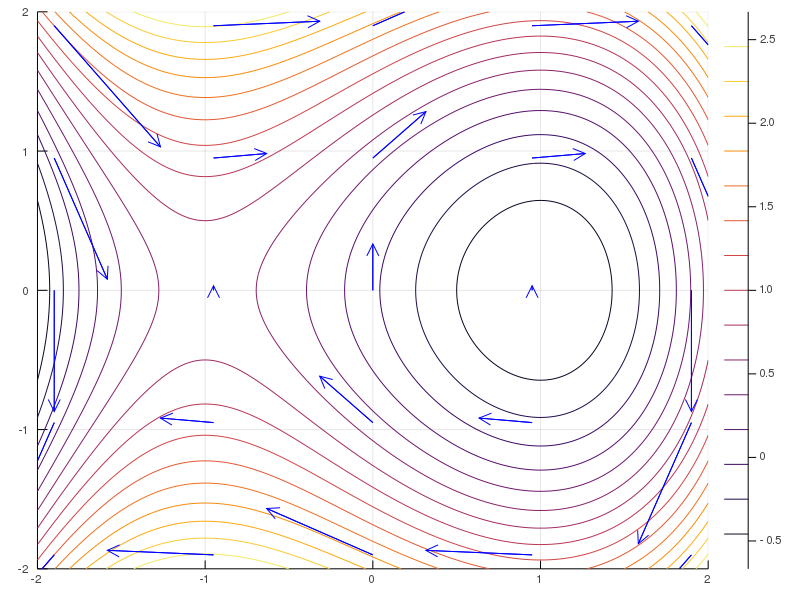
\includegraphics[scale=0.6]{images/vector_space.png}

Now to find the stable points we can just set $\Dot{x} = 0$. This gives us two solutions
\begin{equation}
    x^{(0)} = (1, 0)^T, \ x^{(1)} = (-1, 0)^T 
\end{equation}

To analyze better these points we can take
\begin{equation}
    D \Dot{x} = \begin{pmatrix}
            0 & 1 \\ - 2x_1 & 0
        \end{pmatrix} \\
\end{equation}

And evaluate it the two points.
First, for $x_{(0)}$ we obtain
\begin{equation}
    D \Dot{x}^{(0)} = \begin{pmatrix}
        0 & 1 \\ - 2 & 0
    \end{pmatrix} 
\end{equation}

that has eigen values $\lambda_0^{(0)} = -\sqrt{2}i$ and $\lambda_1^{(0)} = \sqrt{2}i$. This implies that this point is an orbit. Which is validated by the graph.

Likewise, we can evaluate it at $x_{(1)}$,
\begin{equation}
    D \Dot{x}^{(1)} = \begin{pmatrix}
        0 & 1 \\ 2 & 0
    \end{pmatrix} 
\end{equation}

that has eigen values $\lambda_0^{(1)} = -\sqrt{2}$ and $\lambda_1^{(1)} = \sqrt{2}$. This implies that this point is a saddle. \\

Both these results are validated by the Hamiltonian level curves. \\
To see this more clearly let's plot a series of points starting at coordinates $x = (x_1, 0): -1 < x_1 < 1$ against time.

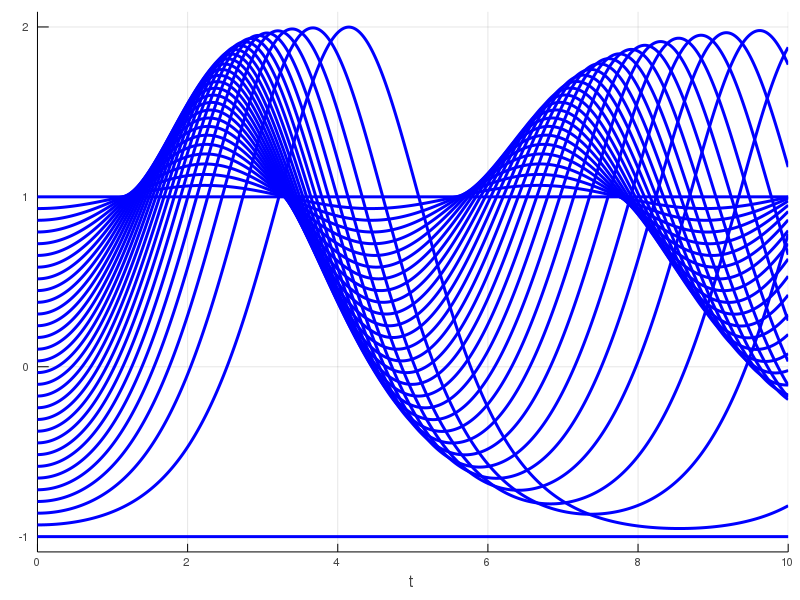
\includegraphics[scale=0.6]{images/manifolds.png}.

We can clearly see that the points at $x_1 = -1 \ and \ x_1 = 1$ stay stable along that axis and the others orbit around $x_1 = 1$. \\

Lastly we can determine the stable and unstable manifolds of the saddle. Another graph could help, here we observe the trajectory of points starting at coordinates $x=(-2, x_2)$ where $x_2$ is in the neighborhood of an approximation of a point lying on the stable manifold (e.g. $1.6329924906907485$), in red. 

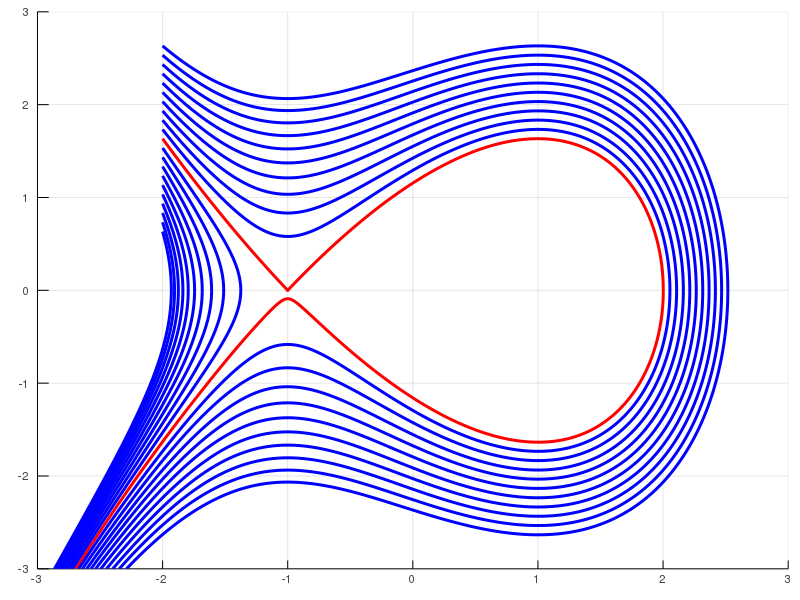
\includegraphics[scale=0.6]{images/stable_manifold_approx.png}

We can clearly see that between the orbit in red and an orbit slightly below it, we will find a stable manifold. \\
In general the manifolds are two. We can talk about them by dividing the plane in four quadrants, delimited by the axis $x_1=-1$ and $x_2 = 0$ First a stable manifold cutting in the second quadrant, with $\Dot{x}_1 > 0 \land \Dot{x}_0 < 0$ approaching the point $(-1, 0)$. Second a stable manifold, represented by the orbit originating at a perturbation of the $(-1, 0)$ towards the first quadrant. This orbit will go around the point $(1, 0)$ and converge into $(-1, 0)$.

\end{homeworkProblem}

\end{document}
